\subsubsection{UC2 - Selezione del grafico per la visualizzazione}
\label{sub:uc2}

\begin{figure}[h]
    \centering
    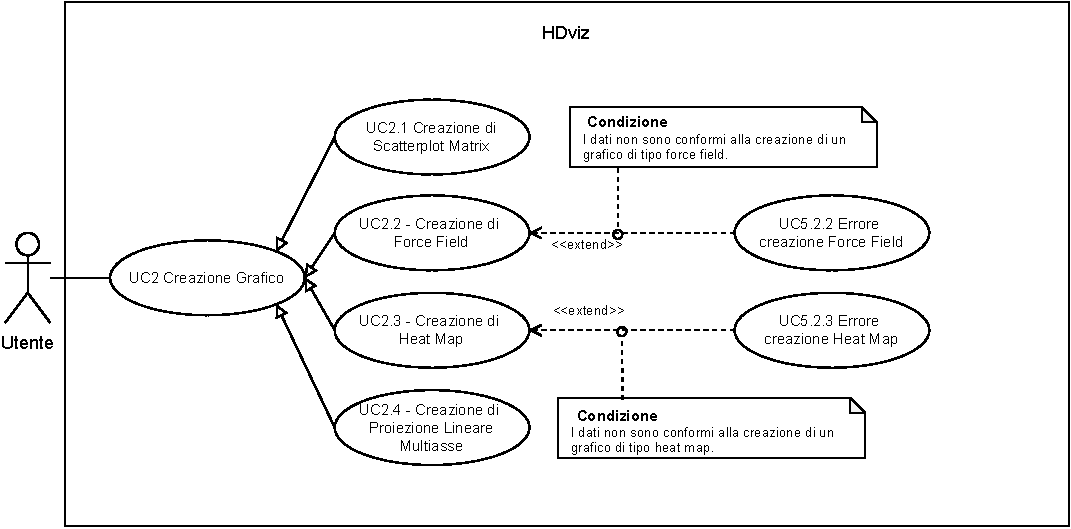
\includegraphics[width=0.5\textwidth]{componenti/casi-duso/diagrammi/UC2.pdf}
    \caption{Diagramma rappresentante UC2}
    \label{fig:UC2}
\end{figure}

\begin{itemize}
	\item \textbf{Descrizione}: L'utente sceglie con quale tipologia di grafico visualizzare i dati;
	\item \textbf{Attore primario}: Utente;
	\item \textbf{Precondizione}: I dati o il progetto sono stati importati correttamente in HD Viz (UC1 \refSec{sub:uc1});
	\item \textbf{Postcondizione}: L'utente ha selezionato con quale tipologia di grafico visualizzerà i dati;
	\item \textbf{Scenario principale}:
		\begin{enumerate}
			\item Vengono mostrati all'utente le tipologie di grafico disponibili dall'applicativo;
			\item L'utente sceglie la tipologia di grafico con cui visualizzare i dati;
		\end{enumerate}
	\item \textbf{Generalizzazioni}: L'utente seleziona una tra le seguenti opzioni:
		\begin{itemize}
			\item \emph{\glossario{Scatter Plot Matrix}} (UC2.1 \refSec{ssub:uc2.1})
			\item \emph{\glossario{Force Field}} (UC2.2 \refSec{ssub:uc2.2})
			\item \emph{\glossario{Heat Map}} (UC2.3 \refSec{ssub:uc2.3})
			\item \emph{\glossario{Proiezione Lineare Multi Asse}} (UC2.4 \refSec{ssub:uc2.4})
		\end{itemize}
\end{itemize}

\paragraph{UC2.1 - Selezionato \emph{Scatter Plot Matrix}}
\label{ssub:uc2.1}

\begin{itemize}
	\item \textbf{Descrizione}: L'utente sceglie \emph{Scatter Plot Matrix} come tipologia di grafico con cui visualizzare i dati;
	\item \textbf{Attore primario}: Utente;
	\item \textbf{Precondizione}: I dati o il progetto sono stati importati correttamente in HD Viz (UC1 \refSec{sub:uc1});
	\item \textbf{Postcondizione}: L'utente ha selezionato \emph{Scatter Plot Matrix} come tipologia di grafico con cui visualizzare i dati;
	\item \textbf{Scenario principale}:
		\begin{enumerate}
			\item Vengono mostrati all'utente le tipologie di grafico disponibili dall'applicativo;
			\item L'utente sceglie \emph{Scatter Plot Matrix} come tipologia di grafico con qui visualizzare i dati;
		\end{enumerate}
\end{itemize}

\paragraph{UC2.2 - Selezionato \emph{Force Field}}
\label{ssub:uc2.2}

\begin{itemize}
	\item \textbf{Descrizione}: L'utente sceglie \emph{Force Field} come tipologia di grafico con cui visualizzare i dati;
	\item \textbf{Attore primario}: Utente;
	\item \textbf{Precondizione}: I dati o il progetto sono stati importati correttamente in HD Viz (UC1 \refSec{sub:uc1});
	\item \textbf{Postcondizione}: L'utente ha selezionato \emph{Force Field} come tipologia di grafico con cui visualizzare i dati;
	\item \textbf{Scenario principale}:
		\begin{enumerate}
			\item Vengono mostrati all'utente le tipologie di grafico disponibili dall'applicativo;
			\item L'utente sceglie \emph{Force Field} come tipologia di grafico con qui visualizzare i dati;
		\end{enumerate}
\end{itemize}


\paragraph{UC2.3 - Selezionato \emph{Heat Map}}
\label{ssub:uc2.3}

	\begin{itemize}
		\item \textbf{Descrizione}: L'utente sceglie \emph{Heat Map} come tipologia di grafico con cui visualizzare i dati;
		\item \textbf{Attore primario}: Utente;
		\item \textbf{Precondizione}: I dati o il progetto sono stati importati correttamente in HD Viz (UC1 \refSec{sub:uc1});
		\item \textbf{Postcondizione}: L'utente ha selezionato \emph{Heat Map} come tipologia di grafico con cui visualizzare i dati;
		\item \textbf{Scenario principale}:
			\begin{enumerate}
				\item Vengono mostrati all'utente le tipologie di grafico disponibili dall'applicativo;
				\item L'utente sceglie \emph{Heat Map} come tipologia di grafico con qui visualizzare i dati;
			\end{enumerate}
	\end{itemize}

\paragraph{UC2.4 - Selezionato \emph{0o}}
\label{ssub:uc2.4}

	\begin{itemize}
		\item \textbf{Descrizione}: L'utente sceglie \emph{Proiezione Lineare Multi Asse} come tipologia di grafico con cui visualizzare i dati;
		\item \textbf{Attore primario}: Utente;
		\item \textbf{Precondizione}: I dati o il progetto sono stati importati correttamente in HD Viz (UC1 \refSec{sub:uc1});
		\item \textbf{Postcondizione}: L'utente ha selezionato \emph{Proiezione Lineare Multi Asse} come tipologia di grafico con cui visualizzare i dati;
		\item \textbf{Scenario principale}:
			\begin{enumerate}
				\item Vengono mostrati all'utente le tipologie di grafico disponibili dall'applicativo;
				\item L'utente sceglie \emph{Proiezione Lineare Multi Asse} come tipologia di grafico con qui visualizzare i dati;
			\end{enumerate}
	\end{itemize}